\section{ProtoDUNE-ND detector physics studies}
\label{sec:detector-physics-studies}
Basic detector stability checks will be checked with a period of detector operation in Bern before moving the module to Fermilab. These tests would include extraction and re-insertion tests of individual modules into the LAr bath, and checks that the LAr purity is sufficient. However, local tests can only be performed using cosmic muons, which have limited utility beyond basic detector stability checks. In this section, we identify a number of key detector physics questions which could be answered by the ProtoDUNE-ND test, and would help inform the final design of the full ArgonCube ND component for DUNE, and aid in developing reconstruction algorithms suitable for neutrino interactions. 
\subsection{Track multiplicity, rate and pile-up}
\begin{figure}[htb]
  \centering
  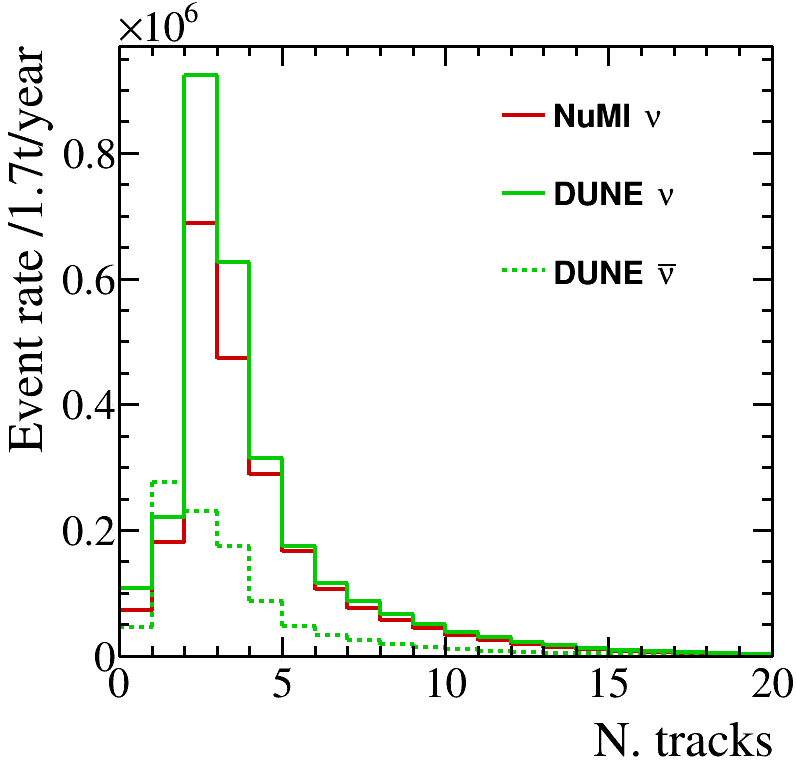
\includegraphics[width=0.5\textwidth]{plots/2x2_ntracks_all.png}
  \caption{The expected yearly rates of minimum and highly ionizing particles expected in the 2x2 module's 1.7t LAr volume for the NuMI ME and LBNF fluxes, produced using GENIE v2.12.8 with the ``ValenciaQEBergerSehgalCOHRES'' configuration~\cite{genie}.}
  \label{fig:track_multiplicity}
\end{figure}
In order to be a relevant test for the full ArgonCube near detector, which will be in the LBNF beamline, it is useful to verify that the basic properties of the events are similar, despite the NuMI ME beam being somewhat higher energy than the planned LBNF beam (as shown in Figure~\ref{fig:beam_options}). Figure~\ref{fig:track_multiplicity} shows the expected multiplicity of minimum or highly ionizing tracks at the vertex for both the LBNF and NuMI ME beams, in neutrino and antineutrino mode, produced with the GENIE generator. The track multiplicities are similar, which indicates that the scale of the reconstruction problem is similar, and the proposed ProtoDUNE-ND test will be a useful benchmark for developing the ArgonCube reconstruction software.

\begin{figure}[htb]
  \centering
  \subfloat[$\mu^{\pm}$] {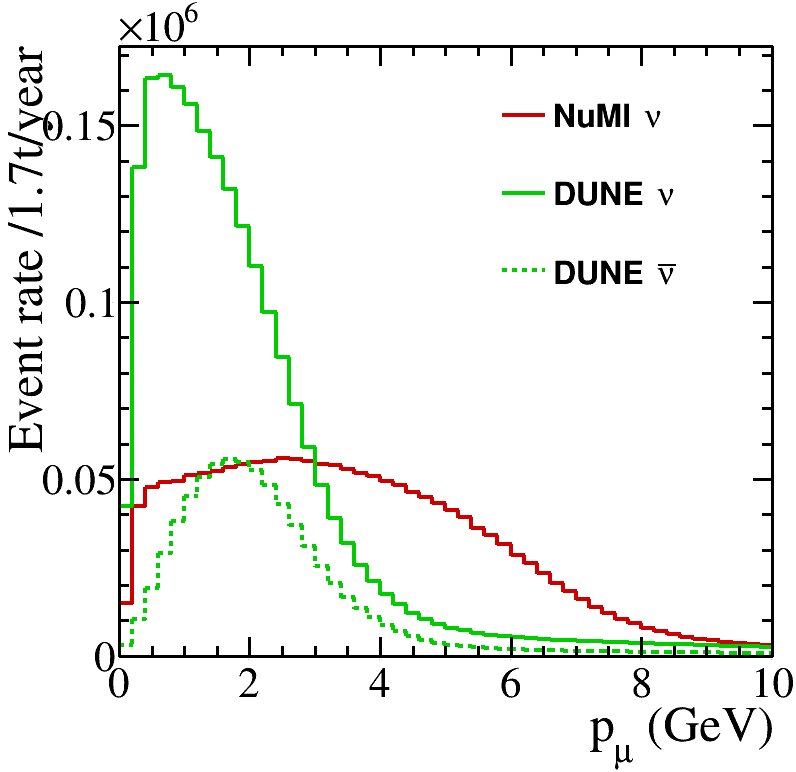
\includegraphics[width=0.5\textwidth]{plots/2x2_muon_mom_all.png}}
  \subfloat[Protons]    {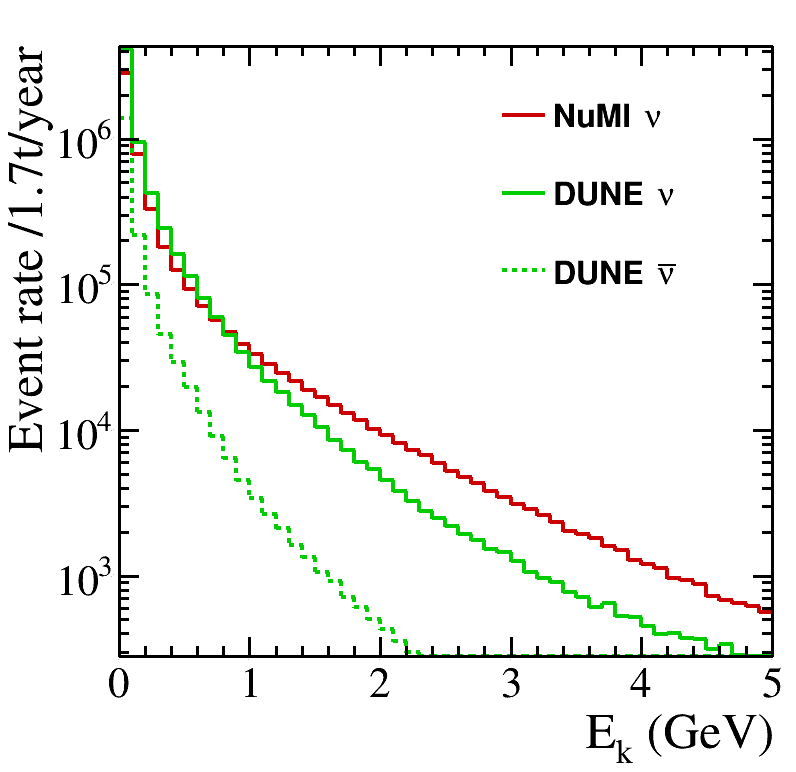
\includegraphics[width=0.5\textwidth]{plots/2x2_proton_Ek_all.png}}\\
  \subfloat[$\pi^{+}$]    {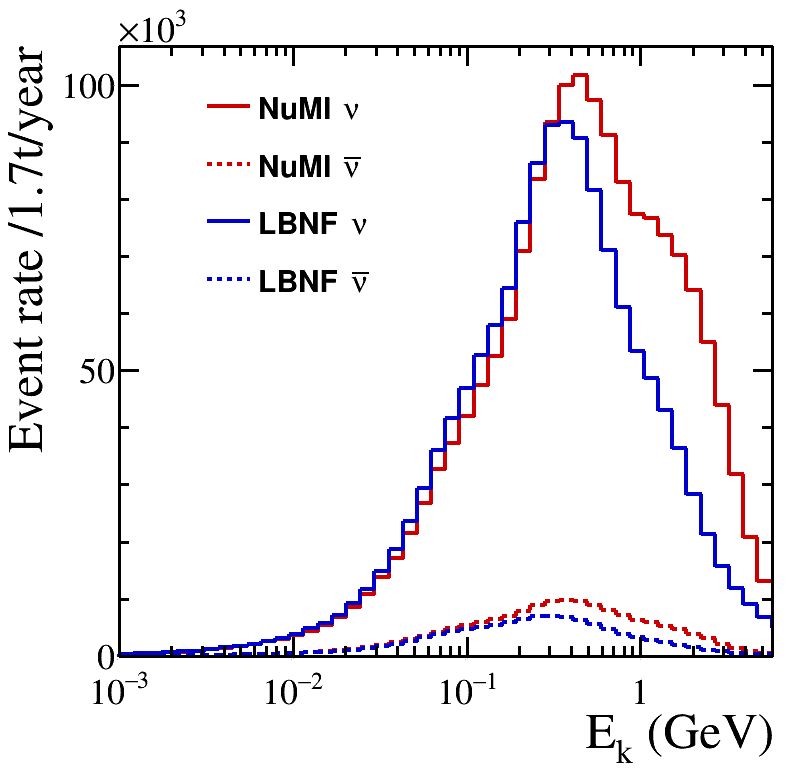
\includegraphics[width=0.5\textwidth]{plots/2x2_piplus_Ek_all.png}}
  \subfloat[$\pi^{-}$]    {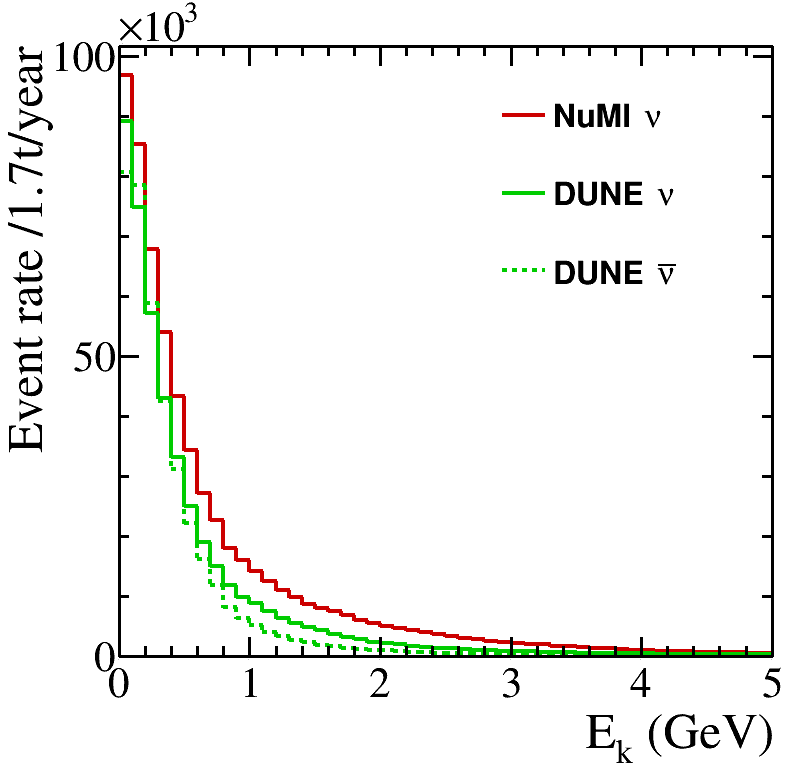
\includegraphics[width=0.5\textwidth]{plots/2x2_piminus_Ek_all.png}}  
  \caption{The expected yearly rates of various particles produced at the vertex, as a function of their kinetic energy, expected in the 2x2 module's 1.7t LAr volume for the NuMI ME and LBNF fluxes, produced using GENIE v2.12.8 with the ``ValenciaQEBergerSehgalCOHRES'' configuration~\cite{genie}. \todo{Get the muon kinetic energy!}}
  \label{fig:kinetic_energies}
\end{figure}
In Figure~\ref{fig:kinetic_energies}, the kinetic energies of various particles coming from the initial neutrino--argon vertex are compared for the LBNF and NuMI ME beams. As expected, the energy distributions of all of the particles are slightly broader for the NuMI ME flux, but there are significant numbers of events with particle kinematics across the broad range of energies expected for the LBNF beams.

In the full ArgonCube detector and the more intense LBNF beamline, pile-up will be a significant challenge



Basic comparisons to DUNE beam, need to add something about pile-up. This section might become a general discussion on what we expect to see in the 2x2. Take Patrick's event displays, show that containment will be an issue, but pile-up won't be.

\FloatBarrier
\subsection{Combining light and charge signals}
An important first test of the detector is how well the prompt light collection efficiency is, and how well the light readout can be combined with charge readout to reconstruct events

\subsection{Identifying neutrons}
\todo{Patrick}

\subsection{Michel tagging efficiency?}
\todo{Figure out if we can do anything remotely reasonable...}

\subsection{Track reconstruction across modules}
\todo{stole this from the LOI}  The module walls produce gaps in particle tracks traversing multiple modules similar to dead wires in classic LArTPC readouts.
Algorithms to join such segmented tracks already exist~\cite{pandora}.
However, a detailed study of the influence of module walls on reconstruction efficiency still needs to be performed.

\subsection{Shower reconstruction across modules}
Charge sharing of EM and hadronic showers between modules. Need Patrick's studies of shower depth, how many showers will be contained, how many not, etc etc

\subsection{Electron-photon separation}
Lots of pi0s, MicroBooNE can't do it well. Build's on Damian's work --> look at his thesis for this.

\subsection{Testing for space charge build-up in a high intensity beam}
\todo{have to tie this to the possible includsion of scintillator paddles}

\subsection{Combining ArgonCube information with downstream detectors}
\todo{Separate argument for using multiple detectors in a ProtoDUNE-ND test. Can argue that using MINERvA/MINOS would also be good...}
